\documentclass[10pt]{article}
\usepackage[letterpaper,textwidth=5.5in,textheight=9in]{geometry}
\usepackage{times}
\usepackage{microtype}
\usepackage{amsmath,amssymb}
\usepackage{booktabs,array,graphicx}
\usepackage[dvipsnames]{xcolor}
\usepackage{enumitem}
\usepackage{caption}
\usepackage[hidelinks]{hyperref}
\captionsetup{font=small,labelfont=bf}
\setlist{nosep,leftmargin=1.25em}
\newcommand{\ca}{\textsc{CrossAudit}}
\newcommand{\risk}{\operatorname{Risk}}
\hypersetup{pdftitle={When Does Independent Audit Help Agentic Research?},pdfauthor={}}

\title{When Does Independent Audit Help Agentic Research?\\
\ca{} and a Causal Evaluation Framework}
\author{Anonymous authors}
\date{}

\begin{document}
\maketitle
\vspace{-1.3em}
\begin{center}
\fcolorbox{BrickRed}{red!4}{\parbox{0.91\linewidth}{\small\textbf{Pre-results draft.}
The protocol, software, sealed six-task feasibility cohort, and prospective
three-vendor design are complete. The 150--180-task human-adjudicated study has
not run. No sentence below treats feasibility or power simulation as efficacy.}}
\end{center}

\begin{abstract}
Language-model agents increasingly generate scientific code, analyses, and
manuscripts, while their review is commonly performed by the same model or
platform. A different vendor may remove exact self-evaluation, but vendor
heterogeneity is neither necessary nor sufficient for independent error. We
introduce \ca{}, a git-native protocol that makes supervision inspectable:
versioned rules, deterministic checks, bounded model revision, fail-closed
admission, and a ledger of findings and dispositions. We formulate the target
as net correction under false-block, revision-harm, model-cost, and human-
attention constraints. A sealed 542-call feasibility cohort on six
deterministic tasks exercised seven measurement paths but produced direction-
specific cross-auditor effects, a circular deterministic ceiling, and no
structured-ledger advantage over an ordinary log on proxy decisions. It does
not establish efficacy. Those failures motivate a prospective study with
150--180 tasks, three vendors, six pinned models, same-model and same-vendor/
different-model controls, three domains, human-blinded gold, and task-clustered
inference. \ca{} contributes an executable protocol and a falsifiable
evaluation of when heterogeneous oversight helps; the positive efficacy claim
is deliberately reserved for the unrun confirmatory study.
\end{abstract}

\section{Introduction}

Agentic research systems can propose hypotheses, execute code, search
literature, and draft papers with limited human intervention
\cite{lu2024,lu2026,gottweis2026}. Their scale changes the supervision problem.
A human can no longer reread every intermediate artefact, yet an automated
reviewer may share the Generator's blind spots. LLM judges exhibit position,
style, and self-preference effects \cite{zheng2023,panickssery2024}; reliable
repetition need not imply valid judgement \cite{norman2026}. At the same time,
the review process is often inaccessible outside a platform.

The tempting remedy is ``use another vendor.'' That intervention removes exact
self-grading, but it bundles several mechanisms: model capability, training and
post-training, prompting infrastructure, data overlap, and stochasticity.
Cross-vendor is therefore an assignment label, not proof of independence. The
scientific question is narrower and testable:

\begin{quote}\small
Under fixed information, budget, and controller rules, when does a more
heterogeneous Auditor improve final artefact quality without unacceptable
clean-artifact burden or revision harm?
\end{quote}

We make four contributions. First, we separate same-model, same-vendor/
different-model, and cross-vendor review. Second, we specify \ca{}, an
executable supervision protocol whose decisions become inspectable artefacts.
Third, we define a causal estimand and operational utility that include false
blocks, new defects, unnecessary changes, model cost, and human attention.
Fourth, we release a prospective three-vendor confirmatory package: allocation,
human adjudication, power simulation, analysis plan, refusal preflight, and
tests. We also report the sealed feasibility cohort that shaped the design,
including its negative boundaries.

The current evidence establishes implementation and measurement feasibility,
not that cross-vendor audit improves science. This distinction is the main
organising choice of the paper.

\section{From same-source concern to a causal question}

Self-preference is documented for some LLM evaluators judging their own
generations \cite{panickssery2024}, but later work shows that quality and
identity blinding can explain part of the measured effect
\cite{chen2025,roytburg2026}. Panel-of-LLM evaluation uses model diversity to
dilute idiosyncratic bias \cite{verga2024}, yet it does not isolate vendor from
model ability. Scientific audit adds asymmetric costs absent from ordinary
ranking: a false block consumes human attention, and a revision can introduce a
new defect.

Let $E_G$ denote a Generator defect and $E_A$ failure by an Auditor to block it.
The relevant association is
\begin{equation}
\rho_{GA}=\operatorname{Corr}(E_G,E_A\mid X,M_G,M_A,H),
\end{equation}
where $X$ is the task, $M_G$ and $M_A$ are resolved model configurations, and
$H$ fixes the harness, prompt, information, and controller. Vendor does not
appear in the definition. It is an assignment attribute that may change
$\rho_{GA}$, auditor capability, both, or neither.

For supervision condition $s$, define
\begin{equation}
U(s)=v_rP_s(R)-c_bP_s(B_0)-c_nP_s(N)-c_uP_s(U)-c_mM_s-c_hH_s,
\label{eq:utility}
\end{equation}
where $R$ is successful repair, $B_0$ an unnecessary block or escalation of a
clean artefact, $N$ a revision-introduced defect, $U$ an unnecessary change,
$M_s$ model cost, and $H_s$ human attention. The weights are deployment-
specific. Unless frozen before results, we report the components and their
Pareto frontier instead of choosing weights post hoc.

This yields four predictions. (i) Same-model, same-vendor/different-model, and
cross-vendor review need not be monotonically ordered. (ii) Deterministic
checks should dominate on decidable defects, but circular evaluation occurs if
the same checker defines gold. (iii) broad rules may increase recall and clean
false blocks together. (iv) hard gates may improve repair while increasing
cost, unnecessary changes, or rule-surface adaptation.

\section{The \ca{} protocol}

Each research increment is a pinned commit in a Science Repository. A
Generator can write that repository but not the Audit Repository. An Auditor
receives the pinned artefact as fenced data, a versioned Constitution, and no
Generator transcript. Deterministic checks run first. The Auditor returns a
schema-valid verdict and rule-cited findings. The controller permits bounded
revision, commits each report and disposition, and escalates unresolved or
invalid states. A verified receipt binds the increment, rulebook, checks,
prompt, and decision. Protected admission should accept only a verified PASS.

\begin{table}[t]
\centering\small\setlength{\tabcolsep}{4pt}
\caption{The eight protocol invariants and their empirical role.}
\label{tab:invariants}
\begin{tabular}{@{}p{13mm}p{47mm}p{59mm}@{}}
\toprule
Invariant & Requirement & Failure it makes measurable \\
\midrule
I1 & declared cross-vendor production audit & exact self-evaluation; not all correlated error \\
I2 & append-only parsed ledger & omitted or overwritten findings \\
I3 & schema and rule-ID validity & confident but ungrounded verdicts \\
I4 & deterministic precedence & model arithmetic or waiver of hard checks \\
I5 & bounded rounds & oscillation and unbounded cost \\
I6 & graded escalation & silent failure versus human interruption \\
I7 & receipt binding & stale rules, prompts, checks, or artefacts \\
I8 & fail-closed admission & audit theatre that refuses no action \\
\bottomrule
\end{tabular}
\end{table}

The present reference implementation does not yet provide the strongest form
of all invariants. It preserves parsed reports rather than raw model exchanges;
vendor identity can be self-declared; the operator can rewrite unpublished git
history; and binding admission to platform branch protection remains a deployer
action. Thus ``third-party-auditable'' presently means internally consistent as
published, not externally anchored or cryptographically attested.

\section{What the sealed feasibility cohort established}

The v4 feasibility cohort used two model configurations and six deterministic
convenience tasks. It scheduled 542 calls across Generator--Auditor assignment,
DCL/Constitution ablations, defensive-production policies, evidence strata,
whole-loop revision, ledger surfaces, and three-repeat integrity cells. An
outcome-free seal preceded scoring. All values below are descriptive and
configuration-specific; the independent sample is six tasks, not 542 calls.

\begin{figure}[t]
\centering
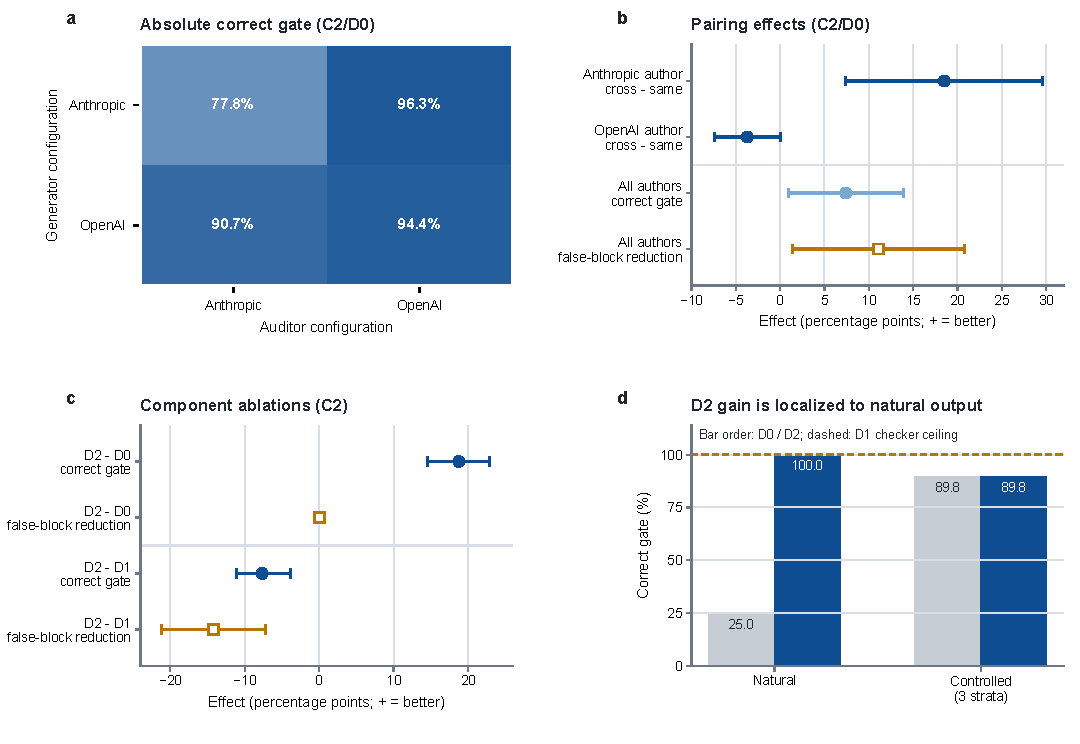
\includegraphics[width=\linewidth]{../../figures/figure5-v4-configuration-effects.pdf}
\caption{Sealed six-task feasibility results. Cross-minus-same correct gating
was positive on average but reversed by Generator direction. Combined DCL plus
model improved over model-only only on natural outputs and remained below the
circular DCL ceiling. Constitution effects are not estimated because the
frozen scorer used repeat 0 where the design called for three repeats.}
\label{fig:feasibility}
\end{figure}

The pooled cross-minus-same correct-gate contrast was $+7.4$ percentage points
and the clean false-block contrast $-11.1$ points. The pooled value concealed
directional changes of $+18.5$ and $-3.7$ points. Combined DCL/model gating was
$+18.8$ points above model-only, entirely on natural outputs, but $-7.6$ points
below DCL-only. The latter checker also defined the micro-task gold labels and
is a harness ceiling, not independent validation.

Across 24 seeded whole-loop branches, same and cross conditions each resolved
12/12 initial defects and ended with 11/12 acceptable artefacts, 1/12 new
defects, and 3/12 unnecessary changes. On seven deterministic episodes, the
structured ledger matched the ordinary log on accept and tamper proxy accuracy
(71.4\% each) and was worse on first-defective-round reconstruction (57.1\%
versus 92.9\%). Proxy reviewers were models, not humans. Hard gating repaired
two of nine initially wrong text outputs without regressing three initially
correct ones, but required more than twice the calls and cost; a two-task code
subset was ceiling-limited and showed compliance-only changes rather than
measured quality gain.

These findings establish that the harness can execute, stop, seal, and measure.
They reject a universal reading of ``cross-vendor is better'' and motivated the
design below. They are not pooled with the confirmatory study, used for observed
power, or promoted to a vendor-population claim.

\section{Prospective confirmatory evaluation}

The v5 package preserves v4 unchanged and begins a new outcome-free design.
The initial sample is 150 independent task briefs, equally blocked over three
domains, with one blinded expansion to at most 180. At least 60 are privacy-
approved real-task or repository replays. Three principal models, one from each
vendor, form a complete Generator $\times$ Auditor matrix. Three alternate
auditor snapshots supply the missing same-vendor/different-model control.

Each task supplies natural principal-model output and, where applicable, a
verified-clean/exactly-one-mutant sibling pair. Unusual but correct artefacts
are hard negatives. Every required cell uses three fresh-context repeats.
Constitution levels C0/C1/C2 each receive three repeats on a balanced 60-task
controlled subset, removing the v4 estimand mismatch. DCL-only gold is created
by independent human or held-out deterministic validation, never by the tested
checker itself.

\begin{table}[t]
\centering\small\setlength{\tabcolsep}{4pt}
\caption{Minimum prospective design and refusal gates.}
\label{tab:design}
\begin{tabular}{@{}p{31mm}p{88mm}@{}}
\toprule
Element & Requirement \\
\midrule
Tasks & 150, three domains, $\geq60$ real replays; blind expansion $\leq180$ \\
Models & 3 vendors, 6 resolved snapshots; complete 3$\times$3 primary matrix \\
Controls & same snapshot, same-vendor/different-model, cross-vendor \\
Human gold & two blinded domain reviewers plus third adjudicator; separate Gold and Matching Panels \\
Calibration & 30 independent items; Krippendorff $\alpha\geq0.80$, raw agreement $\geq0.85$ \\
Primary gate & correct-gate superiority and clean-burden $+5$-point non-inferiority \\
Integrity & provider-returned identity, frozen prompts/tasks/code, external timestamp, outcome-blind 12-task dry run \\
Scope & included configurations only; every direction and leave-one-vendor-out mandatory \\
\bottomrule
\end{tabular}
\end{table}

\subsection{Estimand and inference}

After collapsing repeats and fixed target strata, task $t$ contributes
\begin{equation}
C_t=\frac{1}{3}\sum_g\left[\frac{1}{2}\sum_{a\ne g}Y_{tga}-Y_{tgg}\right].
\end{equation}
The primary point estimate is the mean of $C_t$. Whole-task bootstrap-t
intervals preserve artefacts, siblings, defects, and calls inside the
independent unit. A crossed logistic mixed-effects model with task and base-
artefact intercepts and fixed Generator, Auditor, separation, domain, stratum,
and defect-channel terms is a sensitivity analysis. Vendor is fixed; three
vendors cannot identify a random vendor-population effect.

The headline requires both (i) the lower endpoint of a two-sided 95\% interval
for cross-minus-matched \texttt{correct\_gate} above zero and (ii) the upper endpoint of
a one-sided 95\% interval for clean unnecessary escalation below $+0.05$.
Invalid, missing, or identity-unverified assigned audits are incorrect gates
and clean unnecessary escalations in the service-level intention-to-audit
population. Direction-specific, S1-versus-S0, review-only, DCL-negative,
cost/latency/human-minute, repeat-flip, and leave-one-vendor-out results are
mandatory.

\subsection{Power, cost, and go/no-go}

The simulator mirrors three Generators, natural/clean/mutant artefacts, the
complete 3$\times$3 audit matrix, alternate same-vendor Auditors, task and
base-artefact dependence, and three correlated repeats. It uses no observed v4
outcome. Before dispatch, at least 10,000 datasets per frozen scenario must
show $\geq80$\% conjunctive power at an eight-point effect, calibrated boundary
type-I error, and 93--97\% interval coverage. N=150 failure permits one
prospective increase to 180; N=180 failure converts the paper to estimation or
stops dispatch.

A 10,000-dataset central planning simulation that read no observed outcomes
returned a 7.998-point Monte Carlo marginal effect for the nominal eight-point
scenario, 99.65\% conjunctive power, 94.87\% interval coverage, 2.49\%
directional superiority type-I error, and 4.75\% non-inferiority-boundary type-I
error. This validates the central allocation under the current normal task-
level design interval. The frozen stress scenarios and calibration against the
exact bootstrap-t analysis remain dispatch blockers.

The planned ceiling is 24,930 model calls before separately authorised
technical retries: 450 generations, 12,150 primary audits, 4,050 same-vendor
alternate audits, 6,480 Constitution additions, and about 1,800 whole-loop
calls. The executable preflight refuses dispatch until money, tokens, wall
time, human hours, privacy approval, identity locks, panel calibration, power,
randomisation, and the dry-run receipt are filled and hash-bound. A call ceiling
is not permission to spend.

\section{Defensive adaptation and ledger utility}

Hard rules can improve work or merely reshape it. The confirmatory whole-loop
subset therefore reports final acceptability, resolved defects, new defects,
unnecessary changes, and human minutes rather than treating more assertions,
documentation, or rule citations as quality. Policy P0 hides audit, P1
discloses non-gating shadow audit, and P2 supplies hard-gate findings under the
same maximum rounds. Evidence for harmful defensive programming requires
increased compliance-only or defensive content without improved blinded final
quality or held-out performance. Verbosity alone is not evidence.

Ledger utility is similarly comparative. Human reviewers, not model proxies,
are crossed with episodes under final-only (E0), ordinary transcript (E1), and
structured ledger (E2) surfaces. Primary outcomes are accept/reject accuracy
and time to a correct decision; tamper detection and first-defective-round
reconstruction are secondary. E2 must beat E1, not merely E0, to justify the
structured representation. Unless separately powered and frozen, this module
remains an appendix and cannot rescue the primary audit result.

\section{Limitations and responsible scope}

The protocol audits the research record, not the world. It cannot detect a
miscalibrated instrument, a wrong but accurately described dataset, or fraud
upstream of the repository. Models may share public training corpora across
vendors. A malicious operator can omit failed private runs or rewrite history
before publication. Prompt injection can shape the stochastic report even when
the Auditor is toolless and the DCL is non-overridable. Shipping unpublished
research to another provider creates confidentiality and intellectual-property
obligations outside the protocol.

The confirmatory study, even if positive, supports only its included models,
vendors, domains, task frame, prompts, and controller. Model snapshots age.
Real-task replay can be selected unrepresentatively. Human gold can be wrong;
the calibration gate controls but does not eliminate that risk. The utility
weights in Eq.~\ref{eq:utility} are not universal, so a deployment with costly
false blocks may rationally reject a configuration that improves average gate
accuracy.

\section{Conclusion}

\ca{} makes automated supervision inspectable and falsifiable: deterministic
precedence, rule-cited judgement, bounded revision, receipts, and a versioned
ledger. The sealed feasibility cohort demonstrates the machinery and exposes
why a second vendor cannot be assumed to be a better judge. The prospective
study separates model change from vendor change and evaluates final net
correction under clean-burden and cost constraints. Until it runs, the evidence
supports a protocol and an executable evaluation framework, not efficacy. An
AI scientist should not grade its own homework; this work specifies how to test
whether a different grader actually helps.

\paragraph{Broader impact.} Inspectable audit could reduce silent errors and
make machine-assisted research easier to scrutinise. It could also create false
confidence, centralise rule-making, leak confidential work to providers, or
encourage optimisation to a narrow Constitution. We therefore require explicit
claim scope, human authority over rules and escalations, privacy approval,
negative-result reporting, and visible distinction between measured zero and
unmeasured state.

\begin{thebibliography}{20}\small
\bibitem{lu2024} C.~Lu, C.~Lu, R.~T. Lange, et al. The AI Scientist: Towards fully automated open-ended scientific discovery. arXiv:2408.06292, 2024.
\bibitem{lu2026} C.~Lu, C.~Lu, R.~T. Lange, et al. Towards end-to-end automation of AI research. \emph{Nature}, 651:914--919, 2026.
\bibitem{gottweis2026} J.~Gottweis, W.-H. Weng, A.~Daryin, et al. Accelerating scientific discovery with Co-Scientist. \emph{Nature}, 655:487--496, 2026.
\bibitem{panickssery2024} A.~Panickssery, S.~R. Bowman, and S.~Feng. LLM evaluators recognize and favor their own generations. \emph{NeurIPS}, 2024.
\bibitem{zheng2023} L.~Zheng, W.-L. Chiang, Y.~Sheng, et al. Judging LLM-as-a-judge with MT-Bench and Chatbot Arena. \emph{NeurIPS}, 2023.
\bibitem{norman2026} J.~D. Norman, M.~U. Rivera, and D.~A. Hughes. Reliability without validity: a systematic evaluation of LLM-as-a-judge models. arXiv:2606.19544, 2026.
\bibitem{chen2025} W.-L. Chen, Z.~Wei, X.~Zhu, S.~Feng, and Y.~Meng. Do LLM evaluators prefer themselves for a reason? arXiv:2504.03846, 2025.
\bibitem{roytburg2026} D.~Roytburg, M.~Bozoukov, M.~Nguyen, et al. Are LLM evaluators really narcissists? arXiv:2601.22548, 2026.
\bibitem{verga2024} P.~Verga, S.~Hofstatter, S.~Althammer, et al. Replacing judges with juries: Evaluating LLM generations with a panel of diverse models. arXiv:2404.18796, 2024.
\bibitem{nuijten2016} M.~B. Nuijten, C.~H.~J. Hartgerink, et al. The prevalence of statistical reporting errors in psychology. \emph{Behavior Research Methods}, 48:1205--1226, 2016.
\end{thebibliography}

\end{document}
